\subsection{Reasons of an Overhaul}
\paragraph{}
The original architecture of the vehicle was already a good basis for the
realisation of a line tracking car. However, manual manoeuvring tests by
remote control have revealed some driving faults. Misconduct that could
be embarrassing in an autonomous driving mission. Given that our robot
will certainly not be as adaptive as a human in its driving, it is
interesting to ease the maneuvers and correct some mobility deficiencies.

\subsubsection{Problems identified and changes to be expected}
\paragraph{}
Some of the shortcomings noted are listed as follows:
\begin{itemize}
    \item Loss of control due to high front wheel slippage during high speed turns.
    \item In case of sharp turn, locking of the inner wheel on the bend caused by
    the central component box.
    \item Lack of firmness of the front wheel guiding created by a large backlash.
    \item Uncontrolled spinning of the rear wheels when acceleration from a
    standstill or deceleration from high speeds.
\end{itemize}
And some others component have to be implemented to the initial structure in order
to be an optimal support for autonomous driving such as:
\begin{itemize}
    \item The installation of a camera to see and locate the line to follow.
    \item Hosting a Raspberry Pi card to manage the control computations.
    \item Keep space for the rest of the essential components such as the battery,
    ESC, cables, etc.
\end{itemize}

\subsection{Front Wheel Steering}
\paragraph{}
bla
bla
bla
bla

\begin{figure}[!ht]
    \begin{center}
        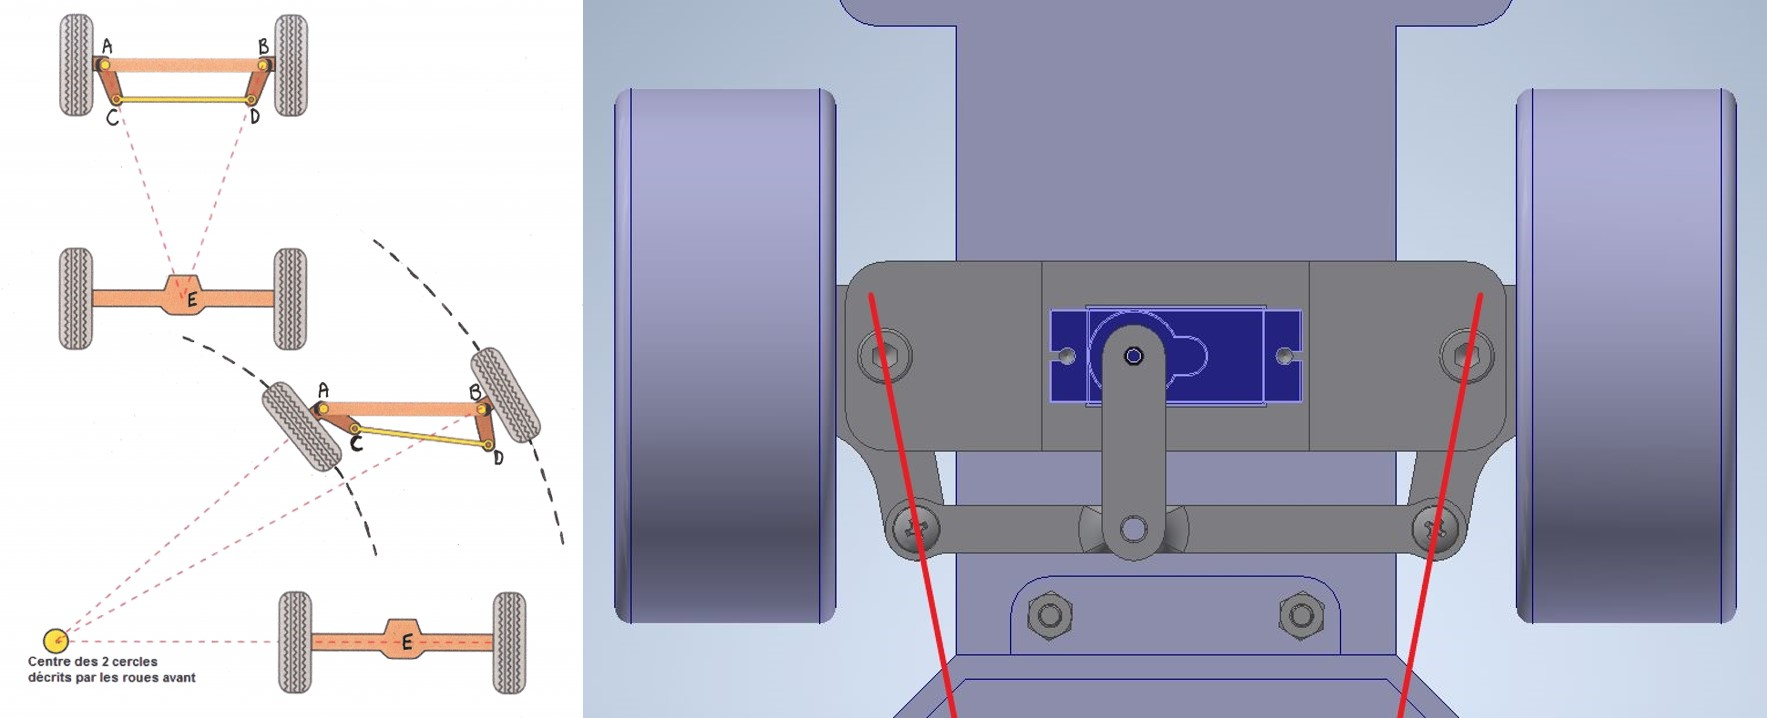
\includegraphics[scale=0.45]{Images/steering.jpg}
    \end{center}
    \caption{Steering system}
    \label{fig:raspi_config}
\end{figure}

\subsection{Front Camera Support}
\paragraph{}
bla
bla
bla
bla

\begin{figure}[!ht]
    \begin{center}
        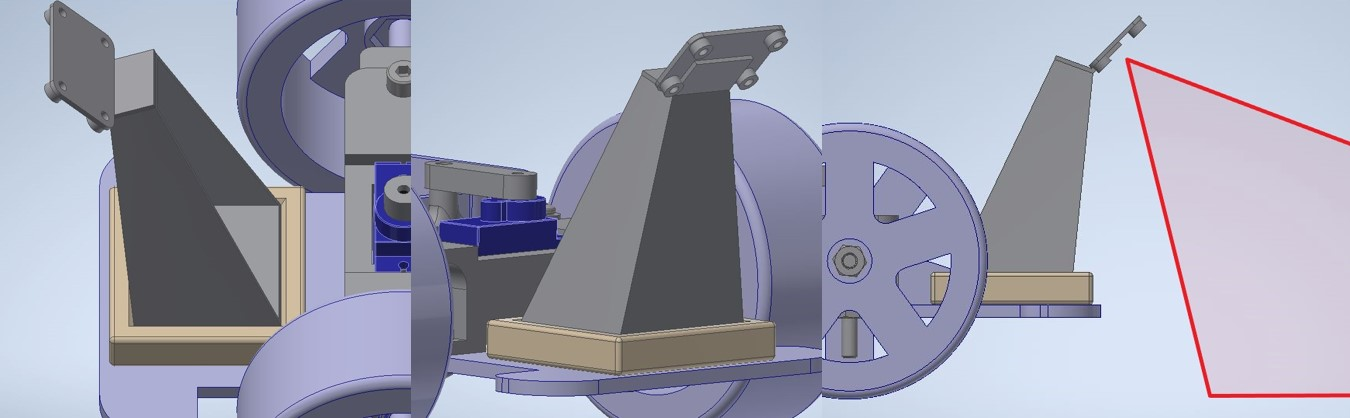
\includegraphics[scale=0.58]{Images/camera_support.jpg}
    \end{center}
    \caption{Front camera support}
    \label{fig:raspi_config}
\end{figure}

\subsection{Component Hosting Box}
\paragraph{}
bla
bla
bla
bla

\begin{figure}[!ht]
    \begin{center}
        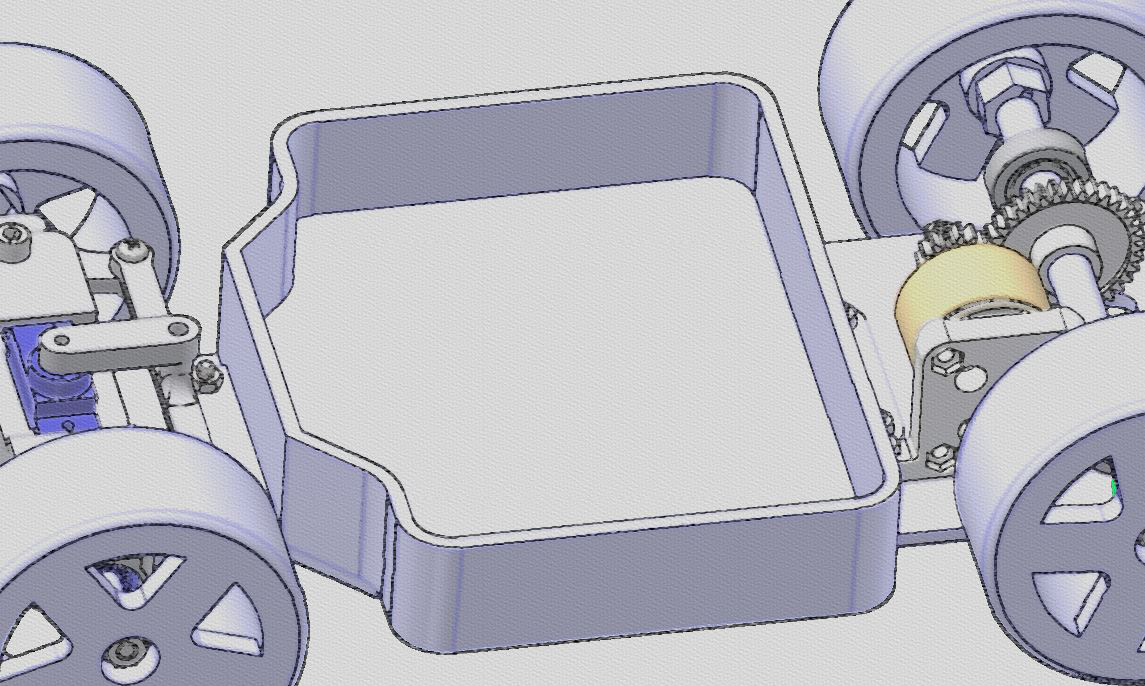
\includegraphics[scale=0.45]{Images/kart_central_box.png}
    \end{center}
    \caption{Central component box}
    \label{fig:raspi_config}
\end{figure}

\subsection{Expectations and Reality}
\paragraph{}
bla bla

\begin{figure}[!ht]
    \begin{center}
        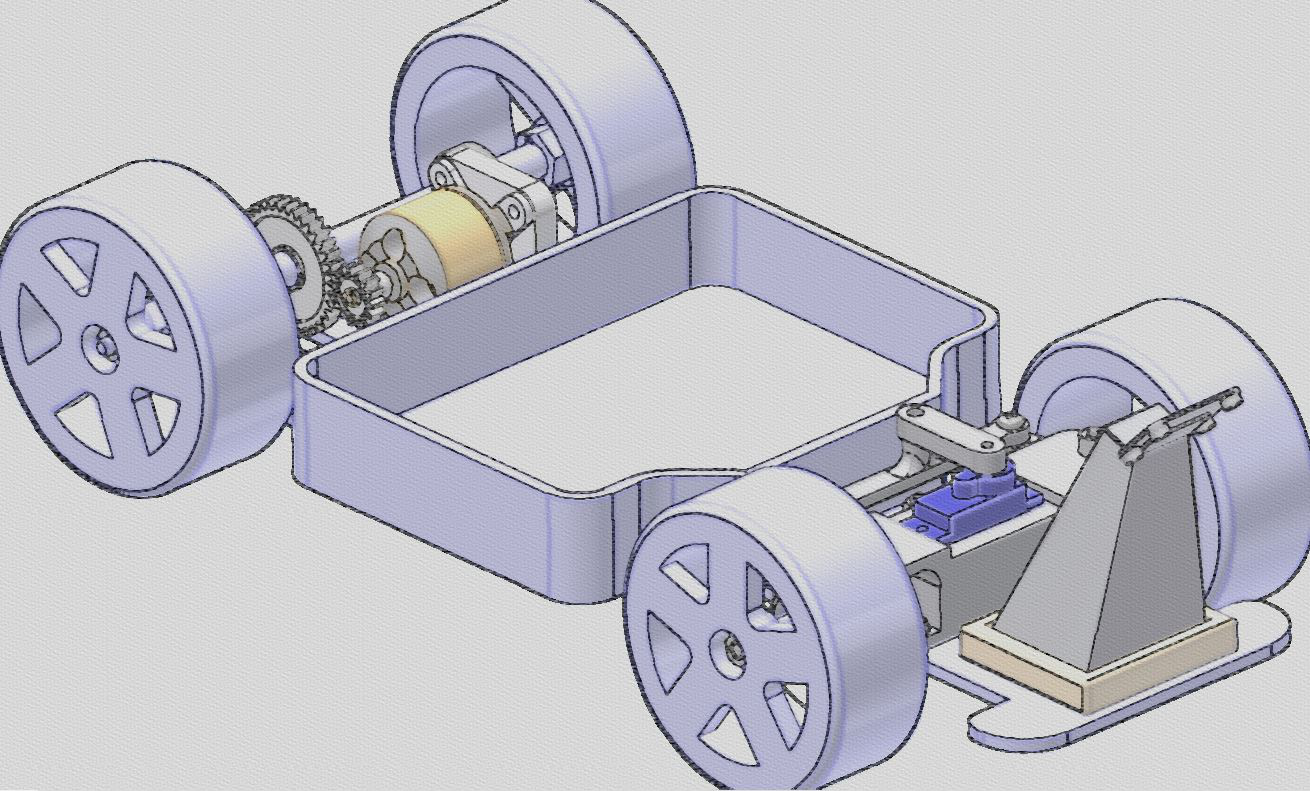
\includegraphics[scale=0.4]{Images/plan_global.png}
        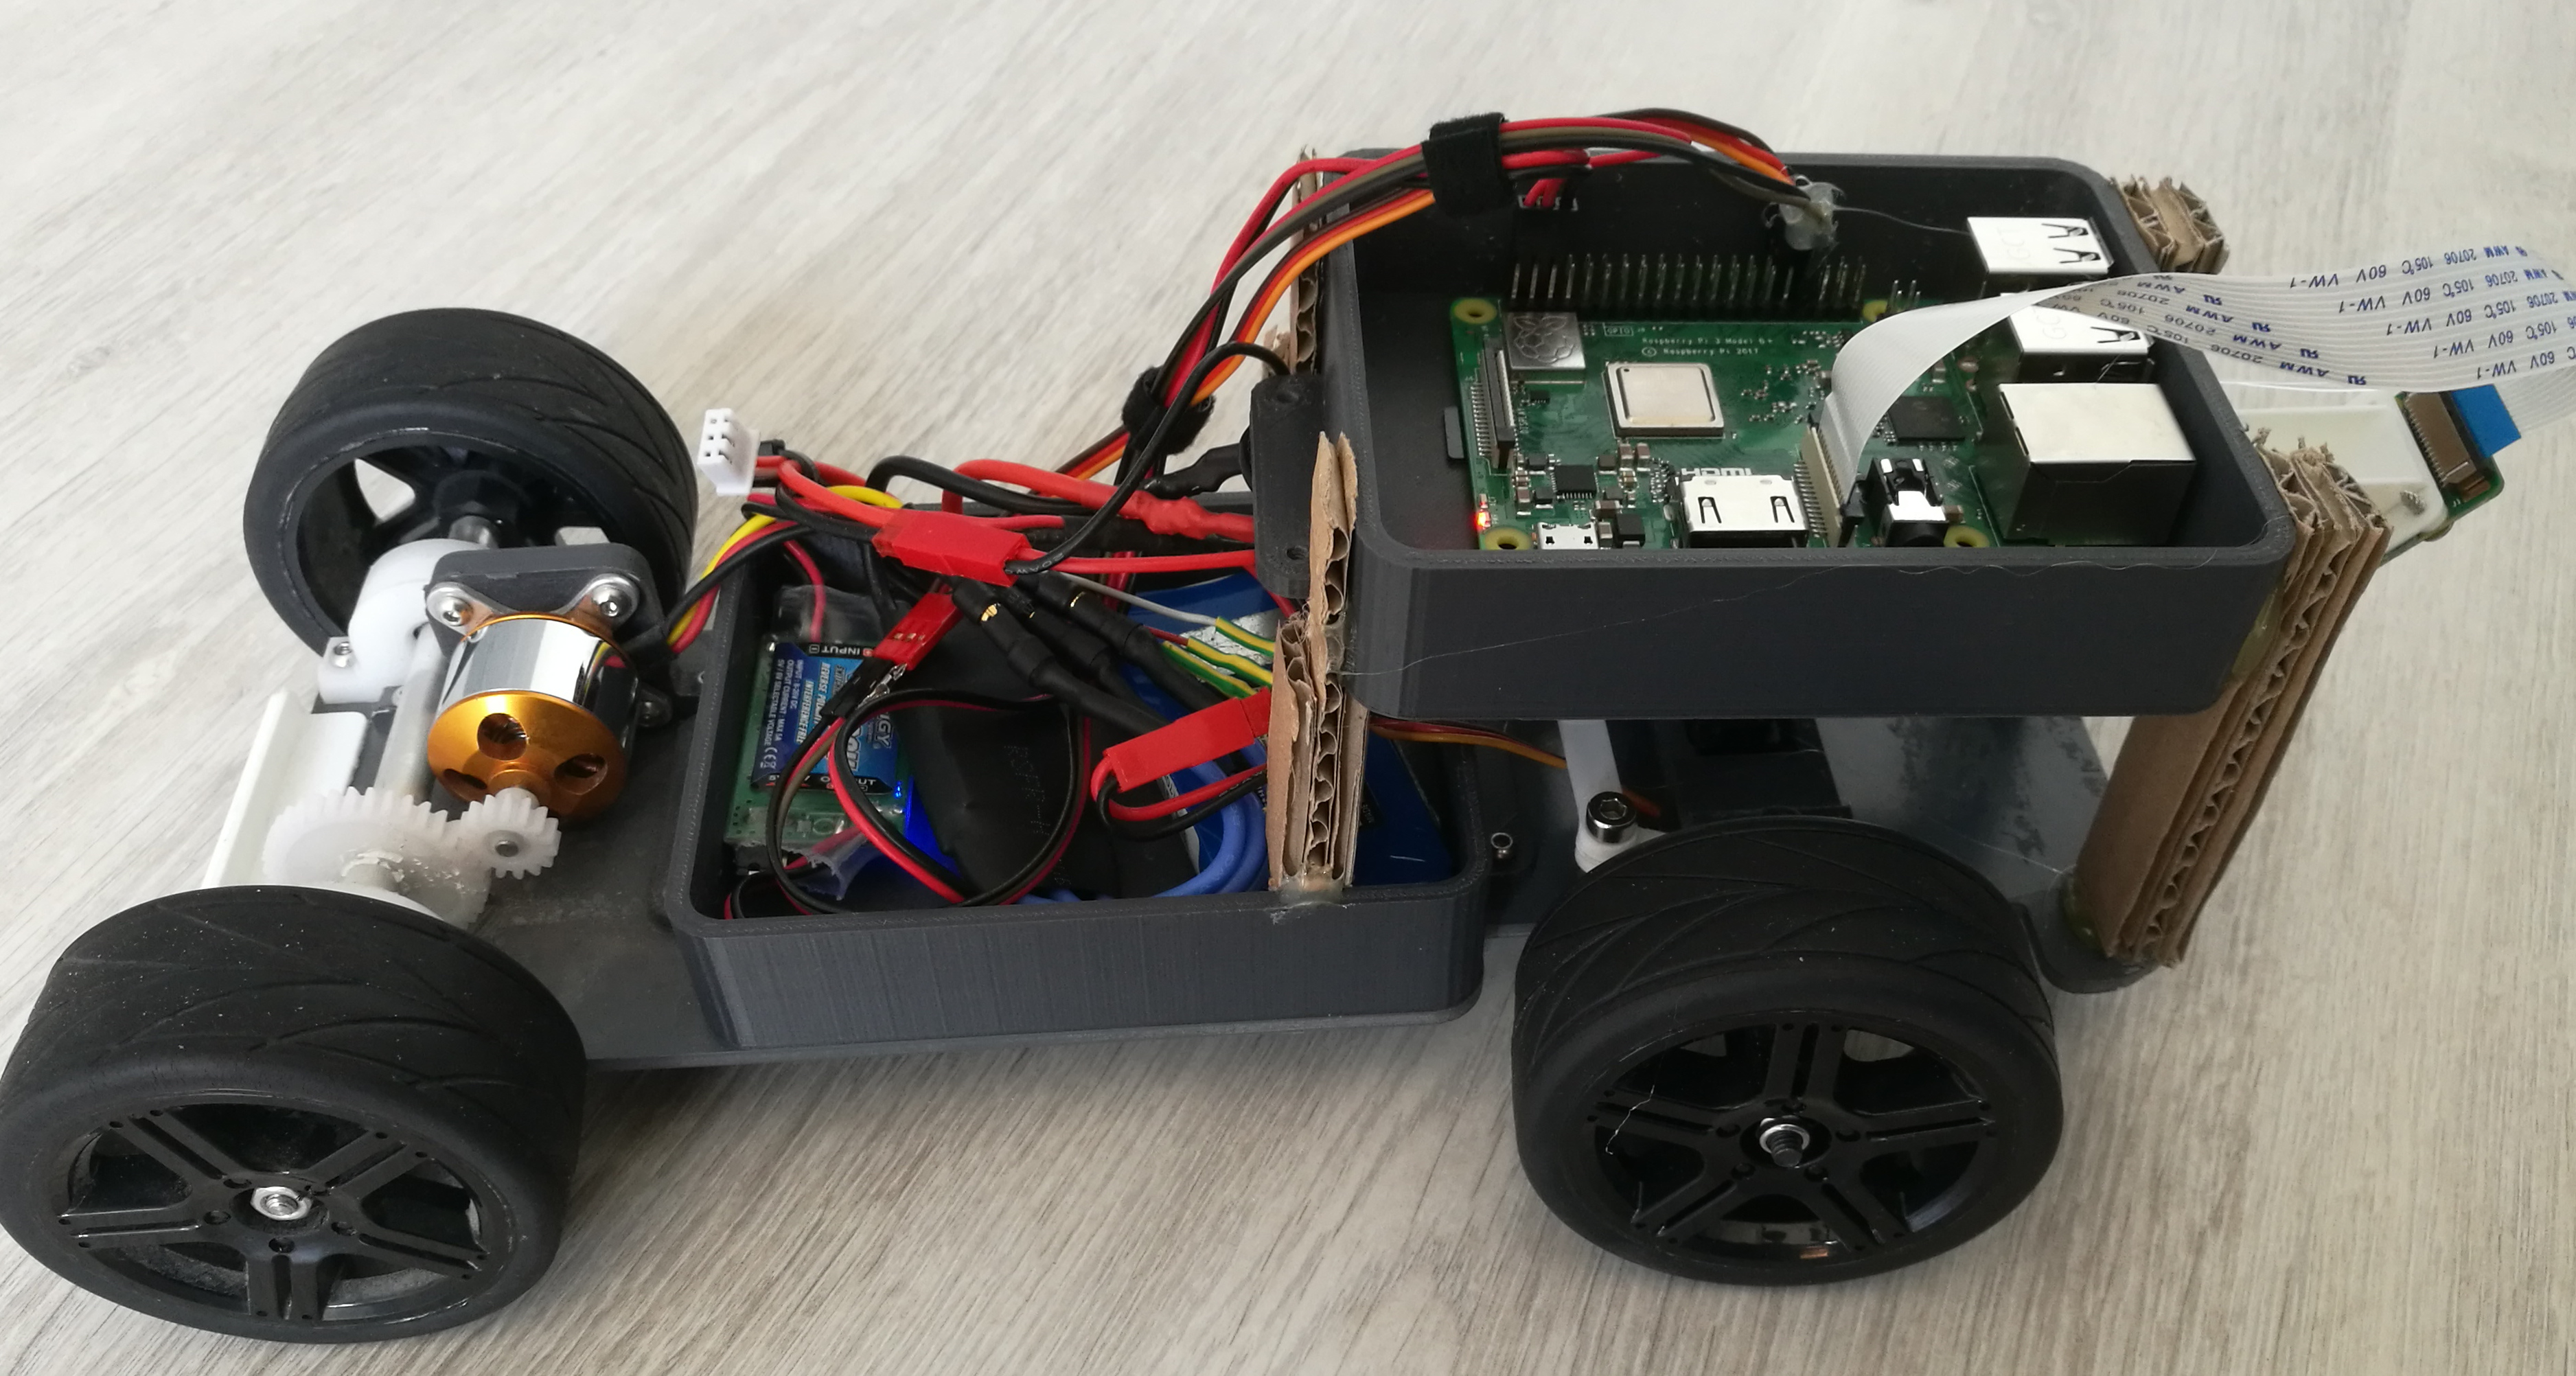
\includegraphics[scale=0.14]{Images/Kart_overview_1.jpg}
    \end{center}
    \caption{Expextations and reality}
    \label{fig:raspi_config}
\end{figure}